\documentclass[11.5pt, twoside, a4paper]{article}
\usepackage{graphicx, amssymb, amsmath, amsthm, xfrac, mathabx, upgreek, fancyhdr, float, underscore, url}
\usepackage[section]{placeins}

\begin{document}

\title{Intelligent Adaptive Systems: Assignment}
\author{Chanelle Lee}
\date{\today}
\maketitle

\section{Introduction}

\subsection{Adaptive Neuro-Fuzzy Inference System (ANFIS)} %Needs a bit more work
ANFIS is a `fuzzy inference system implemented in the framework of adaptive networks' developed in the early 1990s \cite{JangANFIS}. It is called a hybrid neuro-fuzzy technique as it uses the learning capabilities of neural networks to `tune' the membership functions of a Sugeno-type Fuzzy Inference System. 

\subsection{The Task}
The task of this assignment is to use ANFIS to derive a representation of the inverse kinematics of the Lynxmotion robotic arm. In order to investigate this, Matlab's anfis toolbox will be used, with the main questions to be explored:
\begin{enumerate}
\item What is the ideal density of training data? A balance between efficiency and effectiveness is needed; as the more training data points the more accurate the results, but the longer the system takes.
\item How to generate the initial fuzzy inference system; should genfis1 or genfis2 be used? And what parameters should they take?
\item For how many epochs should ANFIS run?
\item What should be the spread of the training data? Should the training data points be uniform over the workspace or concentrated near singularities?
\end{enumerate}

 Due to time constraints, the simpler problem of a two link arm will be used to investigate the first three questions; as the data sets required to train the system are much smaller, and so more exploration of parameter settings of the ANFIS is achievable. Then, the best parameters found will be used to train for a three link arm and as the three link arm gives a planar representation of the Lynxmotion arm, the final question will be investigated. Finally, these findings will be implemented on the Lynxmotion arm and compared against analytical solutions.

\section{Two Link Arm} %should this be link or joint?

For this section, the Lynxmotion arm will be reduced the to the two link problem as described in Fig.\ref{fig:2Link}\footnote{Altered to match findings in Section\ref{sec:elbowIssues}}. 

\begin{figure} %Might be a bit large
\begin{center}
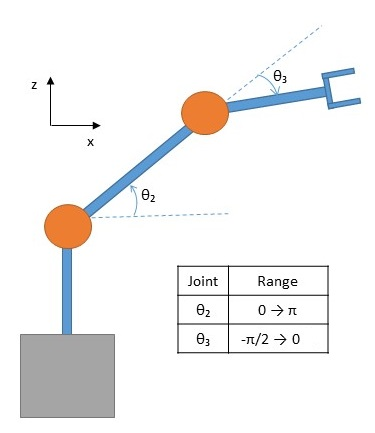
\includegraphics{2Link.jpg}
\caption{Two Link Robotic Arm \label{fig:2Link}}
\end{center}
\end{figure}

\subsection{Joint Angle Range Issues} \label{sec:elbowIssues}

When the experiments were first run there were very large errors in the Cartesian and joint space (Table.\ref{tab:range})\footnote{Genfis1 with two membership functions, 100 data points and 500 epochs.} and this was discovered to be because the range $\theta_3$ was set to $\left[-\pi/2,\pi/2\right]$, This meant that for each point in Cartesian space there were two possible solutions in the joint space with either a positive or negative value for $\theta_3$. This corresponded to the fact that each point in Cartesian space can be reached by the end effector in one of two configurations; elbow up or elbow down. This was solved by limiting the range of $\theta_3$ to only negative values, i.e. limiting the robotic arm to only elbow down configurations, which is much more realistic in terms of the Lynxmotion arm's capabilities.

\begin{table}
\scalebox{0.7}{
\begin{tabular}{|c||c|c|c|c|c|c|c|}\hline
$\theta_3$ range & trnRMSE2 & chkRMSE2 & trnRMSE3 & chkRMSE3 & cartRMSE & cartMin & cartMax\\ \hline\hline
$\left[-\pi/2, \pi/2\right]$ & 0.3792 &  0.3794 &   0.7387  &  0.7389 &  35.7034  &  0.0497 &  99.4345\\ \hline
$\left[-\pi/2, 0\right]$ & 0.0312 &   0.0311  &  0.0682 &   0.0687  &  5.5590  &  0.0651  & 111.7742 \\ \hline
\end{tabular}}
\caption{Results from changing range of $\theta_3$. \label{tab:range}}
\end{table}


\subsection{Number of Epochs}
The number of epochs controls the length of time ANFIS spends tuning the membership functions of the Fuzzy Inference System (FIS) and setting this is a matter of comparing the accuracy attained against the time taken. In Fig.\ref{fig:2000Epochs}\footnote{Genfis1 with two membership functions and 100 data points} it is clear that if only the first fifty epochs are considered the training and validation errors of the joint angles are still falling and there is little evidence to show how far they might further fall, but when one thousand epochs are run there is clearly little improvement after five hundred epochs. Table.\ref{tab:epochs} also shows that the Root-Mean-Squared-Error (RMSE) in the Cartesian space reduces by less than a tenth of a millimetre from five hundred to one thousand epochs despite it taking twice as long to run. Interestingly, there is also little change in the Cartesian RMSE between one hundred epochs and five hundred epochs.. In conclusion, the best number of epochs to use for further experiments is five hundred as confidence can be had that training and validation errors in the joint angles have stabilised by this epoch, but there is little point continuing as neither the error in the joint angles or the Cartesian RMSE appear to decrease enough to be beneficial.

\begin{figure}
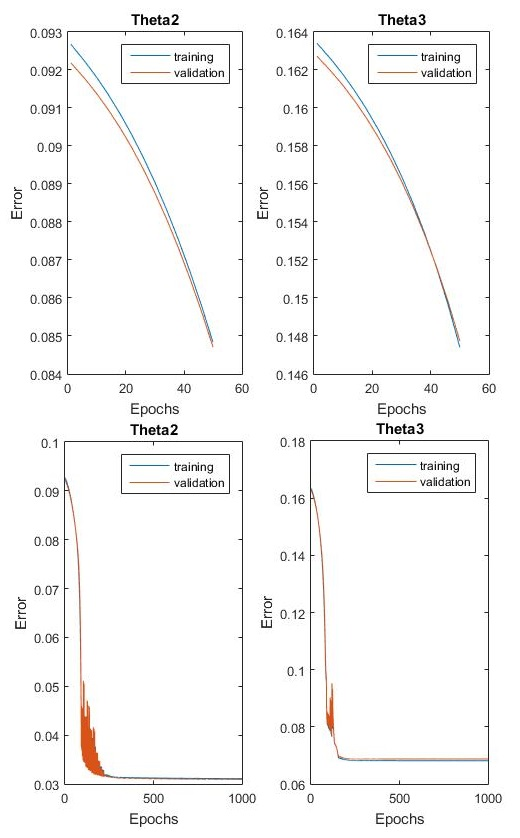
\includegraphics[width=\linewidth]{Epochs.jpg}
\caption{Two Link Arm with run for 50 and 1000 Epochs\label{fig:2000Epochs}}
\end{figure}

\begin{table} 
\scalebox{0.7}{
\begin{tabular}{|c | c | c | c | c | c | c | c | c | c  | c | } 
\hline
dataPoints & Epochs & MFs & trnRMSE2 & chkRMSE2 & trnRMSE3 & chkRMSE3 & cartRMSE & cartMin & cartMax & time \\ \hline \hline
100 &	50   &	2 &	0.0848 &	0.0847 &	0.1474 &	0.1477 &	8.9448 &	0.0728 &	63.0842  &	2.38 \\ \hline
100 &	100  &	2 &	0.0358 &	0.0356 &	0.0795 &	0.0801 &	5.8968 &	0.0425 &	25.2959  &	4.38 \\ \hline
100 &	500  &	2 &	0.0312 &	0.0311 &	0.0682 &	0.0687 &	5.5590 &	0.0651 &	111.7742 &	20.17 \\ \hline
100 &	1000 &	2 &	0.0311 &	0.0309 &	0.0681 &	0.0687 &	5.5723 &	0.0184 &	111.7176 &	39.92 \\ \hline
\end{tabular}}
\caption{Number of Epochs Experiment \label{tab:epochs}}
\end{table}

\subsection{Optimising Genfis1}
To investigate the best parameters using Genfis1 to create the FIS two loops were used to explore:
\begin{itemize}
\item The number of membership functions between two and ten.
\item The number of data points from ten, twenty, fifty, one hundred, two hundred and five hundred.
\end{itemize}
The results from this can be seen in Appendix 1, Table \ref{tab:2LinkGenfis1}; the last half of the two hundred data

\subsubsection{Number of Membership Functions}
The number of membership functions is used by genfis1 to set the number of membership functions of each variable in the FIS \cite{genfis1}. This is important to explore as more membership functions can lead to an increase in accuracy due to a greater capacity for complexity, much like increasing the degree of a polynomial line of best fit. However, too great a capacity for complexity can lead to over-fitting, where the system has been trained so well on the training data, that it is unable to generalise in the areas in between. To continue the polynomial line of best fit example, this would be analogous to increasing the degree of the line of best fit until it passes through every given data point, but in doing so losing the overall shape of the data being described. In order to check for over-fitting, validation data is used so that the error at points not in the training set can be monitored. Then over-fitting can be identified as where the error at training points drops to near zero, but the error at validation points begins to climb, see Figure.\ref{fig:Overfitting}. A countermeasure against over-fitting is to increase the density of the training data, as seen in Figure.\ref{fig:Genfis1}
\begin{figure}
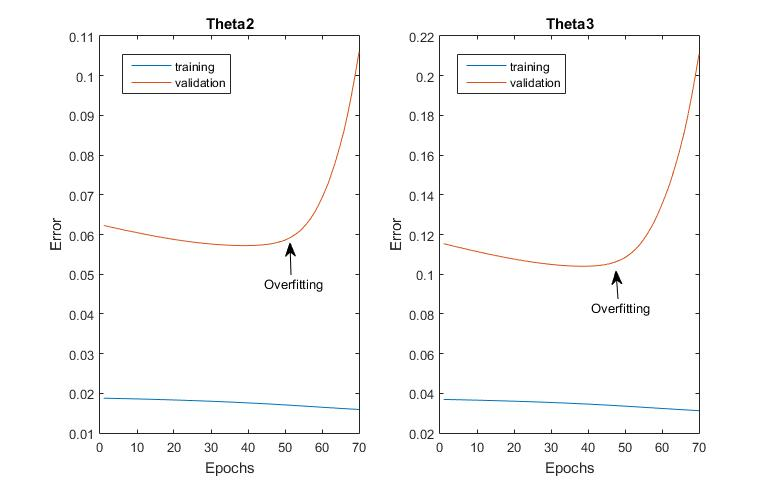
\includegraphics[width=\linewidth]{OverFitting.jpg}
\caption{Example of Over-Fitting\label{fig:Overfitting}}
\end{figure}

Another repercussion of increasing membership functions is that this also increases the time the systems takes to train and so once again a balance needs to be struck between accuracy and efficiency.

\begin{figure}
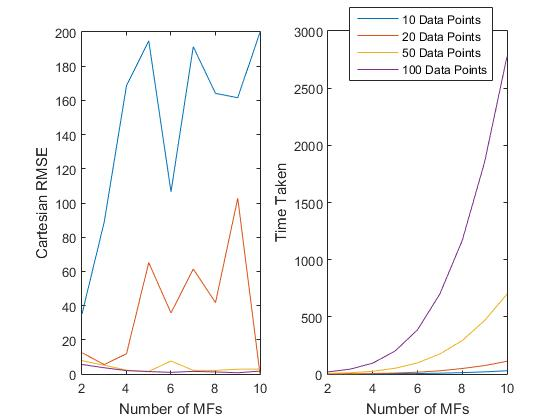
\includegraphics[width=\linewidth]{numMFs.jpg}
\caption{Time and Cartesian RMSE vs Number of Membership Functions for Different Numbers of Data points (from Table \ref{tab:2LinkGenfis1})\label{fig:Genfis1}}
\end{figure}

\subsubsection{Density of Training Data}

A limitation of ANFIS is that it uses supervised learning and as such needs training input-output data, which can be difficult to source for problems and for this task in particular the density of the training data can be a problem. 

\subsection{Optimising Genfis2}
Genfis2 uses subtractive clustering to generate a Sugeno-type FIS structure \cite{genfis2} and in this experiment a genetic algorithm is used to try and determine optimal radii inputs for each joint. A genetic algorithm was chosen here, over any other type of optimisation algorithm, as it was feared that there would be many local optima, e.g. the optimal radius for each cluster. For the sake of convenience, Matlab's built in ga function was used for this experiment; with hard constraints set on the chromosome. However, as genfis2 only accepts radii to one decimal place and the population the ga produces is to four decimal places, the inputs are rounded before genfis2. As the aim of the genetic algorithm is to find the most efficient set of parameters, as opposed to the most accurate, the fitness function used to evaluate the performance of the chromosomes is the Cartesian RMSE mitigated by the time taken.

Time problems were experienced using the genetic algorithm, as the time taken for each generation is the length of time for fitness function (in this case genfis2 and anfis) to run, multiplied by the population size. As such only a small population size of ten was used for this experiment and as such the genetic algorithm converged in a short space of time on a result which may not be globally optimal. In terms of practicality, the length of time necessary to compute the fitness function should in future be taken into account when considering the use of a genetic algorithm. Furthermore, the need to round the chromosomes from Matlab's built-in ga function, meant there was a lot of unnecessary variation within populations.

\section{Three Link Arm}

Need to have another constraint to balance the new variable, using the pitch.

More partitions lead to better results but longer time frame especially the more complicated the system becomes.

\begin{figure}
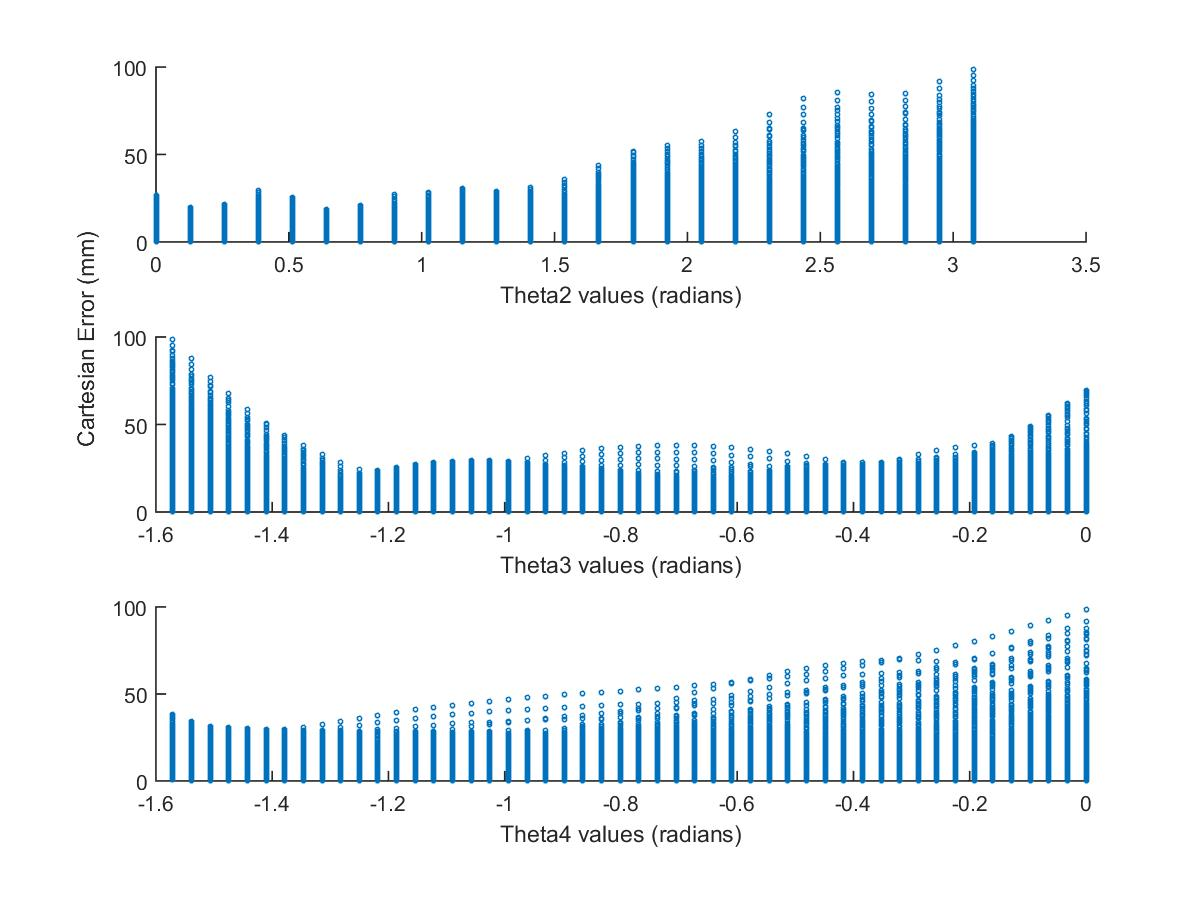
\includegraphics[width=\linewidth]{cartesianerrorsTHETA.jpg}
\caption{Cartesian RMSE in Joint Space\label{fig:carterrors}}
\end{figure}


\section{Lynxmotion Arm}




































\section{Appendix 1 - Experiment Result Tables Overflow}

\begin{table} 
\scalebox{0.7}{
\begin{tabular}{|c | c | c | c | c | c | c | c | c | c  | c | } 
\hline
dataPoints & Epochs & MFs & trnRMSE2 & chkRMSE2 & trnRMSE3 & chkRMSE3 & cartRMSE & cartMin & cartMax & time \\ \hline \hline
10 &	500 &	2 &	0.0441 &	0.1769 &	0.0595 &	0.2102 &	35.0791 &	2.3860 &	151.5126 &		0.32 \\ \hline
10 &	500 &	3 &	0.0075 &	0.6026 &	0.0186 &	1.5039 &	88.9466 &	1.7816 &	300.7353 &		0.44 \\ \hline
10 &	500 &	4 &	0.0016 &	1.5343 &	0.0029 &	2.8815 &	168.6123 &	3.1412 &	464.0428 &		0.99 \\ \hline
10 &	500 &	5 &	0.0005 &	2.3307 &	0.0001 &	1.6801 &	194.8358 &	8.2084 &	519.1364 &		2.03 \\ \hline
10 &	500 &	6 &	0.0000 &	0.7692 &	0.0000 &	1.1000 &	106.5546 &	1.1282 &	342.4532 &		3.91 \\ \hline
10 &	500 &	7 &	0.0000 &	1.0441 &	0.0000 &	1.5253 &	191.3857 &	6.1158 &	625.5818 &		7.09 \\ \hline
10 &	500 &	8 &	0.0000 &	0.8198 &	0.0000 &	0.5227 &	164.0823 &	2.6072 &	624.2153 &		11.81 \\ \hline
10 &	500 &	9 &	0.0000 &	0.8749 &	0.0000 &	0.7083 &	161.5942 &	7.4095 &	629.0190 &		18.56 \\ \hline
10 &	500 &	10 &	0.0000 &	1.0498 &	0.0000 &	0.7715 &	199.8085 &	4.0177 &	629.9484 &		28.28 \\ \hline
20 &	500 &	2 &	0.0487 &	0.0707 &	0.0747 &	0.1185 &	12.4193 &	0.4108 &	103.9274 &		0.74 \\ \hline
20 &	500 &	3 &	0.0196 &	0.0490 &	0.0395 &	0.0945 &	5.5069 &	0.3025 &	24.1058 &		1.74 \\ \hline
20 &	500 &	4 &	0.0204 &	0.0871 &	0.0407 &	0.1851 &	11.8301 &	0.1035 &	64.8913 &		3.95 \\ \hline
20 &	500 &	5 &	0.0083 &	1.0060 &	0.0151 &	1.4404 &	65.1519 &	0.4279 &	462.7651 &		8.43 \\ \hline
20 &	500 &	6 &	0.0037 &	0.1839 &	0.0074 &	0.3333 &	35.6708 &	0.2279 &	256.3560 &		15.52 \\ \hline
20 &	500 &	7 &	0.0018 &	0.3554 &	0.0035 &	0.5666 &	61.4179 &	0.3654 &	572.2944 &		28.16 \\ \hline
20 &	500 &	8 &	0.0013 &	0.2046 &	0.0025 &	0.3664 &	41.7306 &	0.2340 &	212.7630 &		48.13 \\ \hline
20 &	500 &	9 &	0.0011 &	0.3528 &	0.0015 &	0.3827 &	102.7713 &	0.4082 &	488.5110 &		73.61 \\ \hline
20 &	500 &	10 &	0.0007 &	0.3804 &	0.0015 &	0.6136 &	109.5996 &	1.7098 &	521.3018 &		111.39 \\ \hline
50 &	500 &	2 &	0.0371 &	0.0362 &	0.0694 &	0.0769 &	7.7817 &	0.1222 &	98.5986 &		4.46 \\ \hline
50 &	500 &	3 &	0.0248 &	0.0250 &	0.0451 &	0.0512 &	5.1415 &	0.1326 &	99.1554 &		10.80 \\ \hline
50 &	500 &	4 &	0.0206 &	0.0221 &	0.0411 &	0.0435 &	2.2461 &	0.0248 &	13.0735 &		23.72 \\ \hline
50 &	500 &	5 &	0.0164 &	0.0177 &	0.0326 &	0.0348 &	1.5393 &	0.0175 &	7.7383 &		50.42 \\ \hline
50 &	500 &	6 &	0.0124 &	0.0572 &	0.0253 &	0.0767 &	7.5921 &	0.0401 &	209.7884 &		96.92 \\ \hline
50 &	500 &	7 &	0.0112 &	0.0242 &	0.0220 &	0.0487 &	2.1075 &	0.0208 &	23.5713 &		175.22 \\ \hline
50 &	500 &	8 &	0.0103 &	0.0217 &	0.0195 &	0.0383 &	2.1102 &	0.0155 &	22.4959 &		292.86 \\ \hline
50 &	500 &	9 &	0.0087 &	0.0214 &	0.0171 &	0.0451 &	2.8006 &	0.0122 &	26.8913 &		468.32 \\ \hline
50 &	500 &	10 &	0.0081 &	0.0197 &	0.0159 &	0.0394 &	2.8987 &	0.0078 &	45.3157 &		699.17 \\ \hline
100 &	500 &	2 &	0.0312 &	0.0311 &	0.0682 &	0.0687 &	5.5590 &	0.0651 &	111.7742 &		18.10 \\ \hline
100 &	500 &	3 &	0.0236 &	0.0235 &	0.0446 &	0.0458 &	3.6464 &	0.0521 &	29.4106 &		42.97 \\ \hline
100 &	500 &	4 &	0.0200 &	0.0202 &	0.0396 &	0.0400 &	1.9688 &	0.0156 &	10.9047 &		95.06 \\ \hline
100 &	500 &	5 &	0.0158 &	0.0160 &	0.0314 &	0.0318 &	1.4229 &	0.0046 &	14.1410 &		201.28 \\ \hline
100 &	500 &	6 &	0.0117 &	0.0132 &	0.0230 &	0.0261 &	0.9550 &	0.0016 &	8.5618 &		386.25 \\ \hline
100 &	500 &	7 &	0.0105 &	0.0116 &	0.0199 &	0.0211 &	1.5349 &	0.0052 &	19.1859 &		700.12 \\ \hline
100 &	500 &	8 &	0.0100 &	0.0107 &	0.0196 &	0.0212 &	1.1876 &	0.0100 &	35.0601 &		1167.94 \\ \hline
100 &	500 &	9 &	0.0084 &	0.0096 &	0.0163 &	0.0189 &	0.7292 &	0.0023 &	7.2050 &		1854.52 \\ \hline
100 &	500 &	10 &	0.0077 &	0.0107 &	0.0152 &	0.0205 &	1.7005 &	0.0072 &	49.1822 &		2776.96 \\ \hline
200 &	500 &	2 &	0.0300 &	0.0301 &	0.0672 &	0.0675 &	5.6355 &	0.0679 &	168.8529 &		76.53 \\ \hline
200 &	500 &	3 &	0.0236 &	0.0235 &	0.0440 &	0.0441 &	3.2618 &	0.0141 &	21.6430 &		175.64 \\ \hline
200 &	500 &	4 &	0.0197 &	0.0197 &	0.0387 &	0.0388 &	1.8952 &	0.0042 &	11.8753 &		387.51 \\ \hline
200 &	500 &	5 &	0.0146 &	0.0146 &	0.0295 &	0.0295 &	1.6488 &	0.0123 &	8.9011 &		816.60 \\ \hline
200 &	500 &	6 &	0.0114 &	0.0115 &	0.0224 &	0.0226 &	0.8359 &	0.0016 &	6.2123 &		1554.44 \\ \hline
\end{tabular}}
\caption{Two Link Arm - Genfis1 Parameter Experiment \label{tab:2LinkGenfis1}}
\end{table}



\bibliographystyle{unsrt}
\bibliography{IAS}{}


\end{document}